\documentclass[11pt]{article}
\usepackage[a4paper,margin=2.5cm]{geometry}
\usepackage[T1]{fontenc}
\usepackage{newtxtext,newtxmath}
\usepackage{amsmath}
\usepackage{graphicx}
\graphicspath{{../}}
\usepackage{xcolor}
\usepackage[round]{natbib}
\usepackage{xr}
\externaldocument{paper}
\usepackage{hyperref}
\providecommand{\todo}[1]{\textbf{[TODO: #1]}}
\newcommand{\fileref}[1]{\texttt{#1}}
% Generated by docs/build_numbers.py — do not edit by hand.
% Built 2026-09-23T04:26:15+00:00
%
% Any figure the pipeline did not produce renders as \todo{missing},
% so a gap is visible in the PDF rather than filled from memory.
\providecommand{\todo}[1]{\textbf{[TODO: #1]}}

% ---- rangpur_rajshahi ----
\newcommand{\RRAssets}{37,012}
\newcommand{\RRLabelRate}{4.8}
\newcommand{\RRValAUC}{0.886}
\newcommand{\RRValAP}{0.454}
\newcommand{\RRValBrier}{0.131}
\newcommand{\RRValBrierCalibrated}{0.106}
\newcommand{\RRValBrierBaseRate}{0.117}
\newcommand{\RRNCalibration}{2,863}
\newcommand{\RRNTrain}{29,082}
\newcommand{\RRNVal}{5,067}
\newcommand{\RRScoreMean}{0.255}
\newcommand{\RRScoreMedian}{0.14}
\newcommand{\RRKrigingVar}{0.038}
\newcommand{\RRKrigingSillRatio}{0.446}
\newcommand{\RRVariogramRange}{1.605}
\newcommand{\RRNuggetSillRatio}{0.394}
\newcommand{\RRProcessed}{2026-09-23}
\newcommand{\RRNVulnComponents}{4}
\newcommand{\RRObsEvents}{5}
\newcommand{\RRObsFloodedShare}{4.8}
\newcommand{\RRObsAUC}{0.887}
\newcommand{\RRObsAPLift}{3.389}
\newcommand{\RRObsBrierCalibrated}{0.104}
\newcommand{\RRProxyPOD}{0.139}
\newcommand{\RRProxyFAR}{0.518}
\newcommand{\RRProxyCSI}{0.121}
\newcommand{\RRProxyKappa}{0.159}
\newcommand{\RRProxyShare}{4.4}
\newcommand{\RRObservedShare}{15.3}
\newcommand{\RRMinEvents}{2}
\newcommand{\RRSurfaceKrigedObsAUC}{0.574}
\newcommand{\RRSurfaceTerrainObsAUC}{0.709}
\newcommand{\RRProxyTrainedObsAUC}{0.809}
\newcommand{\RRProxyTrainedObsAPLift}{2.382}
\newcommand{\RRCalibBlockRate}{4.2}
\newcommand{\RRTestBlockRate}{13.5}
\newcommand{\RRKrigedGridSD}{0.14}
\newcommand{\RRTerrainGridSD}{0.22}
\newcommand{\RRHazardAUC}{0.76}
\newcommand{\RRHazardAP}{0.184}
\newcommand{\RRHazCoefElevation}{-0.918}
\newcommand{\RRHazCoefSlope}{0.105}
\newcommand{\RRHazCoefTwi}{0.163}
\newcommand{\RRHazCoefHand}{-0.088}
\newcommand{\RRHazCoefFlowAcc}{-0.095}
\newcommand{\RRBenchGraphAUC}{0.795}
\newcommand{\RRBenchGraphSD}{0.038}
\newcommand{\RRBenchGraphLift}{2.88}
\newcommand{\RRBenchLogisticAUC}{0.79}
\newcommand{\RRBenchLogisticSD}{0.04}
\newcommand{\RRBenchLogisticLift}{3.08}
\newcommand{\RRBenchForestAUC}{0.817}
\newcommand{\RRBenchForestSD}{0.046}
\newcommand{\RRBenchForestLift}{3.8}
\newcommand{\RRBenchBoostingAUC}{0.825}
\newcommand{\RRBenchBoostingSD}{0.035}
\newcommand{\RRBenchBoostingLift}{3.57}
\newcommand{\RRBenchTwiAUC}{0.506}
\newcommand{\RRBenchTwiSD}{0.015}
\newcommand{\RRBenchTwiLift}{1.1}
\newcommand{\RRBenchBest}{gradient boosting}
\newcommand{\RRBenchDiff}{-0.03}
\newcommand{\RRBenchGap}{0.03}
\newcommand{\RRBenchDiffP}{0.004}
\newcommand{\RRBenchAhead}{0}
\newcommand{\RRBenchSeeds}{5}
\newcommand{\RRLabelObsAUC}{0.825}
\newcommand{\RRLabelObsSD}{0.035}
\newcommand{\RRLabelProxyAUC}{0.688}
\newcommand{\RRLabelProxySD}{0.045}
\newcommand{\RRLabelGap}{0.137}
\newcommand{\RRLabelGapP}{0}
\newcommand{\RRLabelAhead}{5}
\newcommand{\RRSensEqualTypesRho}{0.96}
\newcommand{\RRSensPopOnlyRho}{0.548}
\newcommand{\RRSensExposureDoubleRho}{0.932}
\newcommand{\RRSensExposureDoubleTop}{0.749}
\newcommand{\RRSensRandomRho}{0.964}
\newcommand{\RRSensRandomRhoMin}{0.919}
\newcommand{\RRSensRandomTop}{0.843}
\newcommand{\RRSensDraws}{20}
\newcommand{\RRNUnions}{1,339}
\newcommand{\RRNUnionsScored}{1,199}
\newcommand{\RRNUpazilas}{148}
\newcommand{\RRNUpazilasScored}{147}
\newcommand{\RRNDistricts}{21}
\newcommand{\RRNDistrictsScored}{21}

% ---- sylhet ----
\newcommand{\SylhetAssets}{17,370}
\newcommand{\SylhetLabelRate}{12.1}
\newcommand{\SylhetValAUC}{0.912}
\newcommand{\SylhetValAP}{0.458}
\newcommand{\SylhetValBrier}{0.086}
\newcommand{\SylhetValBrierCalibrated}{0.064}
\newcommand{\SylhetValBrierBaseRate}{0.089}
\newcommand{\SylhetNCalibration}{2,101}
\newcommand{\SylhetNTrain}{14,006}
\newcommand{\SylhetNVal}{1,263}
\newcommand{\SylhetScoreMean}{0.241}
\newcommand{\SylhetScoreMedian}{0.058}
\newcommand{\SylhetKrigingVar}{0.087}
\newcommand{\SylhetKrigingSillRatio}{0.9}
\newcommand{\SylhetVariogramRange}{0.173}
\newcommand{\SylhetNuggetSillRatio}{0.758}
\newcommand{\SylhetProcessed}{2026-09-23}
\newcommand{\SylhetNVulnComponents}{4}
\newcommand{\SylhetObsEvents}{4}
\newcommand{\SylhetObsFloodedShare}{12}
\newcommand{\SylhetObsAUC}{0.914}
\newcommand{\SylhetObsAPLift}{4.575}
\newcommand{\SylhetObsBrierCalibrated}{0.065}
\newcommand{\SylhetProxyPOD}{0.262}
\newcommand{\SylhetProxyFAR}{0.628}
\newcommand{\SylhetProxyCSI}{0.182}
\newcommand{\SylhetProxyKappa}{0.248}
\newcommand{\SylhetProxyShare}{6.8}
\newcommand{\SylhetObservedShare}{9.6}
\newcommand{\SylhetMinEvents}{2}
\newcommand{\SylhetSurfaceKrigedObsAUC}{0.701}
\newcommand{\SylhetSurfaceTerrainObsAUC}{0.923}
\newcommand{\SylhetProxyTrainedObsAUC}{0.847}
\newcommand{\SylhetProxyTrainedObsAPLift}{3.275}
\newcommand{\SylhetCalibBlockRate}{11.8}
\newcommand{\SylhetTestBlockRate}{9.8}
\newcommand{\SylhetKrigedGridSD}{0.15}
\newcommand{\SylhetTerrainGridSD}{0.27}
\newcommand{\SylhetHazardAUC}{0.807}
\newcommand{\SylhetHazardAP}{0.293}
\newcommand{\SylhetHazCoefElevation}{-22.526}
\newcommand{\SylhetHazCoefSlope}{-0.613}
\newcommand{\SylhetHazCoefTwi}{-0.044}
\newcommand{\SylhetHazCoefHand}{-0.344}
\newcommand{\SylhetHazCoefFlowAcc}{-1.019}
\newcommand{\SylhetBenchGraphAUC}{0.849}
\newcommand{\SylhetBenchGraphSD}{0.016}
\newcommand{\SylhetBenchGraphLift}{3.83}
\newcommand{\SylhetBenchLogisticAUC}{0.81}
\newcommand{\SylhetBenchLogisticSD}{0.06}
\newcommand{\SylhetBenchLogisticLift}{3}
\newcommand{\SylhetBenchForestAUC}{0.875}
\newcommand{\SylhetBenchForestSD}{0.026}
\newcommand{\SylhetBenchForestLift}{4.33}
\newcommand{\SylhetBenchBoostingAUC}{0.872}
\newcommand{\SylhetBenchBoostingSD}{0.028}
\newcommand{\SylhetBenchBoostingLift}{4.13}
\newcommand{\SylhetBenchTwiAUC}{0.581}
\newcommand{\SylhetBenchTwiSD}{0.014}
\newcommand{\SylhetBenchTwiLift}{1.24}
\newcommand{\SylhetBenchBest}{random forest}
\newcommand{\SylhetBenchDiff}{-0.027}
\newcommand{\SylhetBenchGap}{0.027}
\newcommand{\SylhetBenchDiffP}{0.042}
\newcommand{\SylhetBenchAhead}{1}
\newcommand{\SylhetBenchSeeds}{5}
\newcommand{\SylhetLabelObsAUC}{0.872}
\newcommand{\SylhetLabelObsSD}{0.028}
\newcommand{\SylhetLabelProxyAUC}{0.801}
\newcommand{\SylhetLabelProxySD}{0.035}
\newcommand{\SylhetLabelGap}{0.071}
\newcommand{\SylhetLabelGapP}{0}
\newcommand{\SylhetLabelAhead}{5}
\newcommand{\SylhetSensEqualTypesRho}{0.938}
\newcommand{\SylhetSensPopOnlyRho}{0.585}
\newcommand{\SylhetSensExposureDoubleRho}{0.971}
\newcommand{\SylhetSensExposureDoubleTop}{0.742}
\newcommand{\SylhetSensRandomRho}{0.967}
\newcommand{\SylhetSensRandomRhoMin}{0.928}
\newcommand{\SylhetSensRandomTop}{0.829}
\newcommand{\SylhetSensDraws}{20}
\newcommand{\SylhetNUnions}{717}
\newcommand{\SylhetNUnionsScored}{642}
\newcommand{\SylhetNUpazilas}{78}
\newcommand{\SylhetNUpazilasScored}{78}
\newcommand{\SylhetNDistricts}{10}
\newcommand{\SylhetNDistrictsScored}{10}

% ---- sw_coastal ----
\newcommand{\CoastalAssets}{29,829}
\newcommand{\CoastalLabelRate}{4.4}
\newcommand{\CoastalValAUC}{0.783}
\newcommand{\CoastalValAP}{0.063}
\newcommand{\CoastalValBrier}{0.095}
\newcommand{\CoastalValBrierCalibrated}{0.026}
\newcommand{\CoastalValBrierBaseRate}{0.024}
\newcommand{\CoastalNCalibration}{3,274}
\newcommand{\CoastalNTrain}{24,031}
\newcommand{\CoastalNVal}{2,524}
\newcommand{\CoastalScoreMean}{0.193}
\newcommand{\CoastalScoreMedian}{0.053}
\newcommand{\CoastalKrigingVar}{0.052}
\newcommand{\CoastalKrigingSillRatio}{0.82}
\newcommand{\CoastalVariogramRange}{0.157}
\newcommand{\CoastalNuggetSillRatio}{0.559}
\newcommand{\CoastalProcessed}{2026-09-23}
\newcommand{\CoastalNVulnComponents}{4}
\newcommand{\CoastalObsEvents}{4}
\newcommand{\CoastalObsFloodedShare}{4.4}
\newcommand{\CoastalObsAUC}{0.781}
\newcommand{\CoastalObsAPLift}{2.204}
\newcommand{\CoastalObsBrierCalibrated}{0.025}
\newcommand{\CoastalProxyPOD}{0.222}
\newcommand{\CoastalProxyFAR}{0.957}
\newcommand{\CoastalProxyCSI}{0.038}
\newcommand{\CoastalProxyKappa}{0.038}
\newcommand{\CoastalProxyShare}{10.9}
\newcommand{\CoastalObservedShare}{2.1}
\newcommand{\CoastalMinEvents}{1}
\newcommand{\CoastalSurfaceKrigedObsAUC}{0.506}
\newcommand{\CoastalSurfaceTerrainObsAUC}{0.55}
\newcommand{\CoastalProxyTrainedObsAUC}{0.814}
\newcommand{\CoastalProxyTrainedObsAPLift}{3.374}
\newcommand{\CoastalCalibBlockRate}{5.8}
\newcommand{\CoastalTestBlockRate}{2.5}
\newcommand{\CoastalKrigedGridSD}{0.12}
\newcommand{\CoastalTerrainGridSD}{0.38}
\newcommand{\CoastalHazardAUC}{0.773}
\newcommand{\CoastalHazardAP}{0.093}
\newcommand{\CoastalHazCoefElevation}{-1.173}
\newcommand{\CoastalHazCoefSlope}{-0.565}
\newcommand{\CoastalHazCoefTwi}{-0.323}
\newcommand{\CoastalHazCoefHand}{0.073}
\newcommand{\CoastalHazCoefFlowAcc}{-0.181}
\newcommand{\CoastalBenchGraphAUC}{0.824}
\newcommand{\CoastalBenchGraphSD}{0.03}
\newcommand{\CoastalBenchGraphLift}{4.01}
\newcommand{\CoastalBenchLogisticAUC}{0.812}
\newcommand{\CoastalBenchLogisticSD}{0.053}
\newcommand{\CoastalBenchLogisticLift}{4.05}
\newcommand{\CoastalBenchForestAUC}{0.804}
\newcommand{\CoastalBenchForestSD}{0.046}
\newcommand{\CoastalBenchForestLift}{3.82}
\newcommand{\CoastalBenchBoostingAUC}{0.812}
\newcommand{\CoastalBenchBoostingSD}{0.033}
\newcommand{\CoastalBenchBoostingLift}{3.65}
\newcommand{\CoastalBenchTwiAUC}{0.591}
\newcommand{\CoastalBenchTwiSD}{0.037}
\newcommand{\CoastalBenchTwiLift}{1.38}
\newcommand{\CoastalBenchBest}{logistic regression}
\newcommand{\CoastalBenchDiff}{0.012}
\newcommand{\CoastalBenchGap}{0.012}
\newcommand{\CoastalBenchDiffP}{0.513}
\newcommand{\CoastalBenchAhead}{4}
\newcommand{\CoastalBenchSeeds}{5}
\newcommand{\CoastalLabelObsAUC}{0.812}
\newcommand{\CoastalLabelObsSD}{0.033}
\newcommand{\CoastalLabelProxyAUC}{0.781}
\newcommand{\CoastalLabelProxySD}{0.013}
\newcommand{\CoastalLabelGap}{0.031}
\newcommand{\CoastalLabelGapP}{0.08}
\newcommand{\CoastalLabelAhead}{4}
\newcommand{\CoastalSensEqualTypesRho}{0.908}
\newcommand{\CoastalSensPopOnlyRho}{0.42}
\newcommand{\CoastalSensExposureDoubleRho}{0.931}
\newcommand{\CoastalSensExposureDoubleTop}{0.798}
\newcommand{\CoastalSensRandomRho}{0.978}
\newcommand{\CoastalSensRandomRhoMin}{0.962}
\newcommand{\CoastalSensRandomTop}{0.861}
\newcommand{\CoastalSensDraws}{20}
\newcommand{\CoastalNUnions}{943}
\newcommand{\CoastalNUnionsScored}{864}
\newcommand{\CoastalNUpazilas}{99}
\newcommand{\CoastalNUpazilasScored}{99}
\newcommand{\CoastalNDistricts}{16}
\newcommand{\CoastalNDistrictsScored}{16}

% ---- cht ----
\newcommand{\CHTAssets}{\todo{missing}}
\newcommand{\CHTLabelRate}{\todo{missing}}
\newcommand{\CHTValAUC}{\todo{missing}}
\newcommand{\CHTValAP}{\todo{missing}}
\newcommand{\CHTValBrier}{\todo{missing}}
\newcommand{\CHTValBrierCalibrated}{\todo{missing}}
\newcommand{\CHTValBrierBaseRate}{\todo{missing}}
\newcommand{\CHTNCalibration}{\todo{missing}}
\newcommand{\CHTNTrain}{\todo{missing}}
\newcommand{\CHTNVal}{\todo{missing}}
\newcommand{\CHTScoreMean}{\todo{missing}}
\newcommand{\CHTScoreMedian}{\todo{missing}}
\newcommand{\CHTKrigingVar}{\todo{missing}}
\newcommand{\CHTKrigingSillRatio}{\todo{missing}}
\newcommand{\CHTVariogramRange}{\todo{missing}}
\newcommand{\CHTNuggetSillRatio}{\todo{missing}}
\newcommand{\CHTProcessed}{\todo{missing}}
\newcommand{\CHTNVulnComponents}{\todo{missing}}
\newcommand{\CHTObsEvents}{\todo{missing}}
\newcommand{\CHTObsFloodedShare}{\todo{missing}}
\newcommand{\CHTObsAUC}{\todo{missing}}
\newcommand{\CHTObsAPLift}{\todo{missing}}
\newcommand{\CHTObsBrierCalibrated}{\todo{missing}}
\newcommand{\CHTProxyPOD}{\todo{missing}}
\newcommand{\CHTProxyFAR}{\todo{missing}}
\newcommand{\CHTProxyCSI}{\todo{missing}}
\newcommand{\CHTProxyKappa}{\todo{missing}}
\newcommand{\CHTProxyShare}{\todo{missing}}
\newcommand{\CHTObservedShare}{\todo{missing}}
\newcommand{\CHTMinEvents}{\todo{missing}}
\newcommand{\CHTSurfaceKrigedObsAUC}{\todo{missing}}
\newcommand{\CHTSurfaceTerrainObsAUC}{\todo{missing}}
\newcommand{\CHTProxyTrainedObsAUC}{\todo{missing}}
\newcommand{\CHTProxyTrainedObsAPLift}{\todo{missing}}
\newcommand{\CHTCalibBlockRate}{\todo{missing}}
\newcommand{\CHTTestBlockRate}{\todo{missing}}
\newcommand{\CHTKrigedGridSD}{\todo{missing}}
\newcommand{\CHTTerrainGridSD}{\todo{missing}}
\newcommand{\CHTHazardAUC}{\todo{missing}}
\newcommand{\CHTHazardAP}{\todo{missing}}
\newcommand{\CHTLandslides}{1,810}
\newcommand{\CHTBackground}{3,620}
\newcommand{\CHTLSAUC}{0.729}
\newcommand{\CHTLSAP}{0.39}
\newcommand{\CHTCoefElevation}{-0.217}
\newcommand{\CHTCoefSlope}{-0.072}
\newcommand{\CHTCoefTwi}{-0.862}
\newcommand{\CHTCoefHand}{0.291}
\newcommand{\CHTCoefFlowAcc}{0.285}
\newcommand{\CHTBenchGraphAUC}{\todo{missing}}
\newcommand{\CHTBenchGraphSD}{\todo{missing}}
\newcommand{\CHTBenchGraphLift}{\todo{missing}}
\newcommand{\CHTBenchLogisticAUC}{\todo{missing}}
\newcommand{\CHTBenchLogisticSD}{\todo{missing}}
\newcommand{\CHTBenchLogisticLift}{\todo{missing}}
\newcommand{\CHTBenchForestAUC}{\todo{missing}}
\newcommand{\CHTBenchForestSD}{\todo{missing}}
\newcommand{\CHTBenchForestLift}{\todo{missing}}
\newcommand{\CHTBenchBoostingAUC}{\todo{missing}}
\newcommand{\CHTBenchBoostingSD}{\todo{missing}}
\newcommand{\CHTBenchBoostingLift}{\todo{missing}}
\newcommand{\CHTBenchTwiAUC}{\todo{missing}}
\newcommand{\CHTBenchTwiSD}{\todo{missing}}
\newcommand{\CHTBenchTwiLift}{\todo{missing}}
\newcommand{\CHTBenchBest}{\todo{missing}}
\newcommand{\CHTBenchDiff}{\todo{missing}}
\newcommand{\CHTBenchGap}{\todo{missing}}
\newcommand{\CHTBenchDiffP}{\todo{missing}}
\newcommand{\CHTBenchAhead}{\todo{missing}}
\newcommand{\CHTBenchSeeds}{\todo{missing}}
\newcommand{\CHTLabelObsAUC}{\todo{missing}}
\newcommand{\CHTLabelObsSD}{\todo{missing}}
\newcommand{\CHTLabelProxyAUC}{\todo{missing}}
\newcommand{\CHTLabelProxySD}{\todo{missing}}
\newcommand{\CHTLabelGap}{\todo{missing}}
\newcommand{\CHTLabelGapP}{\todo{missing}}
\newcommand{\CHTLabelAhead}{\todo{missing}}
\newcommand{\CHTSensEqualTypesRho}{\todo{missing}}
\newcommand{\CHTSensPopOnlyRho}{\todo{missing}}
\newcommand{\CHTSensExposureDoubleRho}{\todo{missing}}
\newcommand{\CHTSensExposureDoubleTop}{\todo{missing}}
\newcommand{\CHTSensRandomRho}{\todo{missing}}
\newcommand{\CHTSensRandomRhoMin}{\todo{missing}}
\newcommand{\CHTSensRandomTop}{\todo{missing}}
\newcommand{\CHTSensDraws}{\todo{missing}}
\newcommand{\CHTNUnions}{\todo{missing}}
\newcommand{\CHTNUnionsScored}{\todo{missing}}
\newcommand{\CHTNUpazilas}{\todo{missing}}
\newcommand{\CHTNUpazilasScored}{\todo{missing}}
\newcommand{\CHTNDistricts}{\todo{missing}}
\newcommand{\CHTNDistrictsScored}{\todo{missing}}


\renewcommand{\thesection}{S\arabic{section}}
\renewcommand{\thefigure}{S\arabic{figure}}

\title{Supporting Information for ``Do flood susceptibility models know more than the flood record? Evidence from radar-observed floods in Bangladesh''}
\author{Md Rakib Hasan}
\date{}

\begin{document}
\maketitle

This file gives the pipeline settings with a map of the two hazard surfaces (Fig.~S1), the construction of the composite risk and the sensitivity of its weights, which the main text summarises. Section, figure and table numbers without the prefix S refer to the main text. The code that produces every number here is at \url{https://github.com/rakibhhridoy/rimes-mapathon}, and the data at \url{https://doi.org/10.5281/zenodo.22978729}.

\section{Pipeline and model settings}
\label{si:settings}

\subsection*{Infrastructure, terrain and features}

Assets are fetched from the Overpass API by bounding box, in tiles of 0.75$^\circ$, and clipped to the region afterwards. Tiling avoids the timeouts that a query for a whole division produces. Three tag groups are requested, with lifeline assets covering hospitals, clinics, schools, colleges, shelters, bridges, embankments and dams, transport assets covering primary to trunk roads, railways and tagged bridges, and agricultural assets covering farmland, aquaculture, canals, ditches and marketplaces. Each feature is classified into one asset type from its tags and labelled with the district it falls in.

The SRTM tiles covering the bounding box are merged, reprojected to UTM zone 46N and clipped. From the projected elevation model the pipeline derives slope, the topographic wetness index (TWI), height above nearest drainage (HAND) and D8 flow accumulation. Drainage cells for HAND are those above the 90th percentile of flow accumulation, and HAND is the elevation difference between each cell and the nearest drainage cell found by a distance transform.

For each asset the pipeline samples the five terrain rasters at its representative point, samples WorldPop density, and computes the distance in metres to the nearest hospital, school, flood shelter, road and irrigation channel. Asset type enters as a categorical code, all features are standardised to zero mean and unit variance, and the label is the flood-prone status of the ground under the asset. Sampling reprojects the query coordinates into each raster's coordinate system before reading it, and the pipeline stops if any feature comes out constant or if the labels contain a single class.

\subsection*{Asset model, graph and calibration}

The model that scores assets is a configuration setting, \texttt{asset\_model.type}, and the default is class-weighted gradient boosting over the asset features, at 300 boosting iterations with a learning rate of 0.1. That default follows from the comparison in Section~\ref{sec:benchmark}, which found ordinary tabular models matching or beating the graph network the system began with. The graph network remains available, as a two-layer GraphSAGE with 64 hidden channels and dropout of 0.3, trained with a class-weighted loss and early stopping on the calibration blocks, and so do a random forest and logistic regression. In the two riverine regions the scores shown on the map come from the same model given one more feature, the share of earlier Sentinel-1 events in which the ground flooded, trained to predict the flooding of the latest event year from the years before it and applied with the share over every event (Section~\ref{sec:temporal}). Every validation figure in this paper comes from the model without that feature, because the feature is built from the same events the models are scored against.

Assets also form the nodes of a $k$-nearest-neighbour graph with $k=6$, where any pair further apart than 5\,km, measured in metres in the projected coordinate system, is left unconnected. Inverse-distance weights are stored with each edge, although the GraphSAGE mean aggregation does not use them, so every retained neighbour counts equally. Under the default model the edges carry nothing and the graph serves only to hold the features, labels and block assignment that every model shares.

Validation holds out whole spatial blocks of 10\,km instead of random nodes, because neighbouring assets share terrain, so a random split leaves every validation node next to training nodes that carry almost the same features and label, and the resulting score measures memorisation rather than skill. Blocks are assigned at random with a fixed seed to three groups, with 80\,\% for training and the remainder split evenly between calibration and test. Early stopping and the isotonic calibration of the scores use the calibration blocks only, and every metric reported in this paper comes from the test blocks, which neither has seen. Isotonic regression returns the observed frequency of each level it fits, so a level holding a handful of calibration points that all flooded returns a probability of one. Each level is therefore shrunk by its Jeffreys estimate, $(k+0.5)/(n+1)$ for $k$ of $n$ points flooded, which leaves a level carrying many points almost unchanged and pulls a level carrying few back towards the middle. In Rangpur and Rajshahi the raw scores give a Brier score of \RRValBrier{} on the test blocks and the calibrated probabilities \RRValBrierCalibrated{}, against \RRValBrierBaseRate{} for always predicting the base rate, so the calibration corrects the inflated raw scores but adds little over the base rate. Flood prevalence differs from one set of blocks to another, which limits how far a calibration carries. In Rangpur and Rajshahi \RRCalibBlockRate{}\,\% of the assets in the calibration blocks sit on flood-prone ground against \RRTestBlockRate{}\,\% in the test blocks, and a calibration fitted on the first set therefore underestimates the second (Fig.~\ref{fig:calibration}). The calibrated value is best read as an approximate probability for the region as a whole, reliable in its ranking but not in its level for any one area.

\subsection*{Hazard surfaces}

Two hazard surfaces are produced for every flood region, and the composite risk uses one of them according to the configuration setting \texttt{risk.hazard\_source}. The first is ordinary Kriging of the model scores at the asset locations, with a spherical variogram fitted on up to 3,000 points and a residual Kriging pass that adds back the score residuals at the nodes. How much it can say between assets depends on the spatial structure of the scores, which the fitted variogram reports. The nugget is the share of the variance that is unexplained at zero distance, and the mean Kriging variance over the full sill is the share the interpolation leaves unexplained on average. On the current runs the nugget is \RRNuggetSillRatio{} of the sill in Rangpur and Rajshahi and \SylhetNuggetSillRatio{} in Sylhet, and the mean Kriging variance is \RRKrigingSillRatio{} and \SylhetKrigingSillRatio{} of the sill respectively, so in both regions the interpolated surface smooths substantially towards the regional average. In Rangpur and Rajshahi its standard deviation across the grid is \RRKrigedGridSD{} against \RRTerrainGridSD{} for the terrain surface described next, and it varies smoothly over tens of kilometres where the terrain surface follows individual channels and levees (Fig.~\ref{fig:hazard}).

The second surface is a class-weighted logistic regression from each grid cell's own terrain, using elevation, slope, TWI, HAND and flow accumulation and nothing else, because distances to hospitals or roads describe exposure and vulnerability rather than the likelihood of flooding. It is trained at the asset locations on the same labels and the same spatial blocks as the asset model, and evaluated at every grid cell, so it varies at the resolution of the elevation model rather than at the spacing of mapped infrastructure. In Rangpur and Rajshahi it reaches an AUC of \RRHazardAUC{} on held-out blocks, and it is the default. The two surfaces can also be scored directly against observed flooding over every grid cell, not only at assets, and there the terrain surface reaches an AUC of \RRSurfaceTerrainObsAUC{} against \RRSurfaceKrigedObsAUC{} for the Kriged one. Both are written to the grid so the difference between them can be inspected. Because the terrain model is trained on the observed extents, it is a flood-probability surface fitted to what the radar saw. Were it trained on the proxy labels instead, the circularity described in Section~\ref{sec:labels} would apply with full force, and it would be no more than ground the ensemble calls flood-prone, smoothed into a probability.

\begin{figure}[t]
\centering
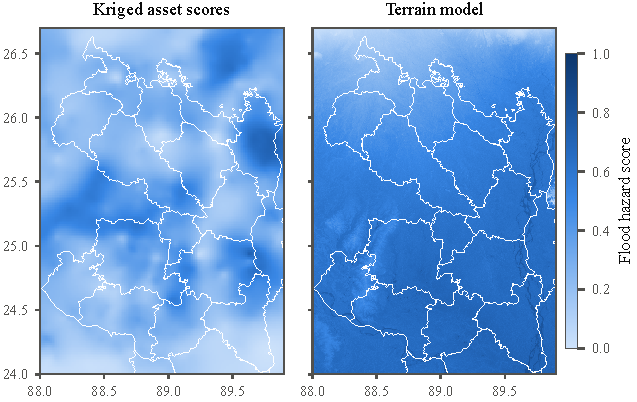
\includegraphics[width=\textwidth]{figures/fig_hazard_surfaces.pdf}
\caption{The two flood hazard surfaces for Rangpur and Rajshahi, with district boundaries in white. The Kriged surface interpolates the asset model's scores between mapped assets and has a standard deviation of \RRKrigedGridSD{} across the grid. The terrain model scores each 30\,m cell from its own elevation, slope, TWI, HAND and flow accumulation, has a standard deviation of \RRTerrainGridSD{}, and reaches a cell-level AUC against observed flooding of \RRSurfaceTerrainObsAUC{}, against \RRSurfaceKrigedObsAUC{} for the Kriged surface.}
\label{fig:hazard}
\end{figure}

\section{Exposure, vulnerability, composite risk and aggregation}
\label{si:risk}

Exposure per cell is measured twice, because ``where is infrastructure at risk'' and ``where would people be affected'' are different questions with different answers. Infrastructure exposure is the type-weighted count of mapped assets in the cell, with hospitals and schools weighted at 0.20, bridges, roads and cropland at 0.15, shelters and embankments at 0.10 and other assets at 0.05, log-scaled to the unit interval. Population exposure is WorldPop density sampled at the cell centre, log-scaled the same way. Urban municipalities lead the first measure because that is where infrastructure is concentrated, while crowded floodplain settlements can lead the second.

Vulnerability combines population density with the distance from the cell centre to the nearest hospital, flood shelter and primary road, each normalised so that a greater distance means greater vulnerability. The configuration lists further components, a night-light proxy and an elderly-and-child ratio, that have no data source yet. Components without data are excluded rather than filled with a constant, and the remaining weights renormalised, and the weights actually applied are written to the output directory alongside the results. For the current runs the four applied components are population density (0.40), distance to hospital (0.27), distance to shelter (0.20) and distance to road (0.13).

Composite risk is the geometric mean of hazard, exposure and vulnerability, which keeps the multiplicative logic, in which no exposure means no risk, while staying on the unit scale of its inputs. Two composites are written, one for each exposure measure, and both are carried through to the administrative summaries. Because the composite is bounded by its weakest factor it rarely approaches 1 even where risk is locally worst, so fixed cut-offs would place almost every cell in the lowest class. Cells are therefore also assigned relative classes 1 to 5 by quintile of the non-zero composite, the usual practice for susceptibility maps. Class 0 marks cells with no mapped exposure, which is an absence of data, not an absence of risk.

Grid results are summarised for every union, upazila and district from geoBoundaries, and each summary carries the mean and maximum of both composites, counts of exposed assets by type, and a flag stating whether the unit holds any mapped assets at all, and units without mapped assets have their risk left undefined. In Rangpur and Rajshahi \RRNUnionsScored{} of the \RRNUnions{} unions hold mapped assets and carry a score. Unit names repeat across Bangladesh, so each unit also carries a label naming its parent, such as ``Abdullahpur (Gangachara)''. Hotspots are detected with the Getis--Ord $G_i^*$ statistic on $k=8$ nearest-neighbour weights, at 95\,\% confidence, over the cells that carry non-zero composite risk. Restricting the statistic to those cells keeps the weights matrix small enough to compute and avoids treating the empty majority of the grid as a sea of low values against which any occupied cell would look hot. Figure~\ref{fig:unionrisk} maps the mean composite risk of every union in the three flood regions.

\section{Sensitivity of the composite to its weights}
\label{si:sensitivity}

The composite risk rests on weights that were chosen rather than measured, so the ranking it produces is recomputed under other defensible choices and compared with the published one by Spearman correlation and by the share of the top decile of cells that stays in the top decile. Weighting every asset type equally leaves the ordering almost unchanged, at $\rho=\RRSensEqualTypesRho{}$ in Rangpur and Rajshahi and $\rho=\CoastalSensEqualTypesRho{}$ on the coast, and so does weighting the vulnerability components equally. Doubling the exposure exponent in the geometric mean gives $\rho=\RRSensExposureDoubleRho{}$ while retaining \RRSensExposureDoubleTop{} of the top decile. Multiplying every chosen weight by a random factor between 0.5 and 1.5, over \RRSensDraws{} draws, gives a mean $\rho$ of \RRSensRandomRho{} in Rangpur and Rajshahi, \SylhetSensRandomRho{} in Sylhet and \CoastalSensRandomRho{} on the coast, with \RRSensRandomTop{} of the top decile retained.

Only one choice matters, reducing vulnerability to population density alone, which discards the distances to hospitals, shelters and roads and drops the correlation to \RRSensPopOnlyRho{} in Rangpur and Rajshahi and \CoastalSensPopOnlyRho{} on the coast, so the access distances rather than population drive the vulnerability term. The ordering of cells is therefore not an artefact of the particular weights, while the boundary of the top class is soft enough that a cell just inside it and a cell just outside should be treated alike.

\section{Validation metrics}
\label{si:metrics}

Every model in the chain is scored on spatial blocks held out from training, and the same block assignment is shared by the asset model and the terrain hazard model within a region. Metrics are the area under the ROC curve, which measures ranking, average precision, which is more sensitive to the rare positive class, and the Brier score for calibration. Average precision is also reported as a lift over the base rate, because an average precision of 0.07 against a positive rate of 0.01 is a sevenfold improvement over chance while the same value against a rate of 0.10 is worse than chance.

The validation step then answers three questions separately. Whether model scores rank assets that flooded above those that did not is measured on the held-out blocks. Whether the hazard surface agrees with observed flooding across the whole grid, and not only where assets happen to be, is measured by AUC and Spearman correlation over all cells. And how closely the proxy labels match observed flooding is measured with the categorical scores used in flood mapping, the probability of detection, false alarm ratio and critical success index, which quantifies what the proxy-trained models were learning.

Every metric that compares two models or two label sources is repeated over several block assignments drawn with different seeds, because a single assignment gives one number with no sense of its spread, and differences are tested by a paired comparison across assignments. Each such comparison uses \RRBenchSeeds{} assignments.


\bibliographystyle{apalike}
\bibliography{references}

\end{document}
